\section{Machine learning-based compression}
\label{sec:machine_learning}

As discussed in the previous sections, any mechanism which can detect regularities in a stream of data and predict future observations (symbols) from past ones (context) can also be used for compression by using it to estimate the probabilities of potential future observations and using these to assign shorter codes to the most likely of them.

While n-gram language models are very simple and easy to train, they are limited by their pre-specified (and often short) context, namely the previous [n-1] symbols in a text, with symbols being either characters or full words. For this reason, statistical models such as n-gram language models have generally been superseded by neural network-based models such as recurrent neural networks (RNNs), long short-term memory models (LSTMs), and most recently large language models (LLMs) such as BERT and GPT, which can retain information across larger contexts and better capture long-range dependencies in a text.

For RNNs, this is accomplished by having the network's previous outputs act as additional inputs when it observes a new symbol, giving it a simple form of memory. An improvement on this model is LSTMs, which are a subtype of RNNs that can learn to select relevant information to keep within its memory, and which generally outperform simple RNNs. Lastly, transformer-based LLMs use an attention mechanism to weight the relative importance of all words in the input data when making a prediction.

In this section I perform simple experiments with one simple RNN and one LSTM. To do this, I create a subclass of \texttt{Predictor} named \texttt{NNPredictor}, which is a predictor that uses a neural network to learn regularities in text. \texttt{RNNPredictor} and \texttt{LSTMPredictor} classes are then created as subclasses of \texttt{NNPredictor}, each specifying its architecture. These are then plugged (along with entropy codings) into \texttt{Compressor} objects. The code for this section can be found at \texttt{\href{https://github.com/Guy29/FYP/blob/main/Code/machine_learning}{Code/machine\_learning}}.

As before, it is possible to feed the \texttt{decode} method noise to see what regularities the model has learned about.

\begin{figure}[h]
\centering
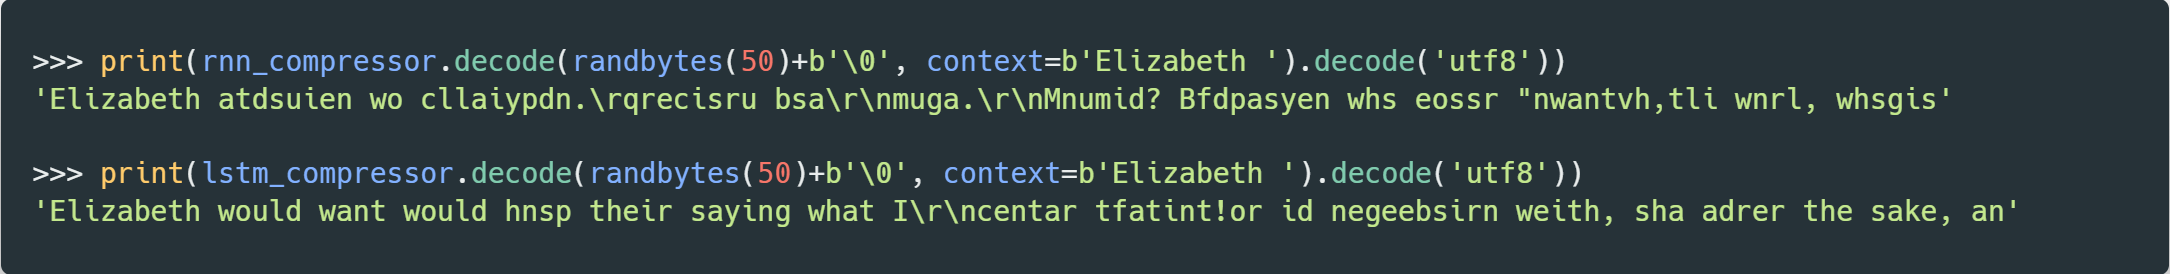
\includegraphics[width=\textwidth]{img/ML_decoding_randomness.png}
\caption{Using the \texttt{decode} method on a randomly generated input}
\label{fig:ML_decoding_randomness}
\end{figure}

With both models the text is much less coherent than with the n-gram model, although the models have still learned which byte values are characters, how often spaces are used, some common collocations, and in the case of the LSTM model some common words. It is likely that with more training or a wider context window the models would be better able to capture the regularities in English, but due to constraints on time and computational power it was not possible to test this in more depth.

As part of the process of training, my code serializes and saves the models periodically. One of the significant advantages of machine learning models over n-gram based models is that the trained version is much smaller (approximately 4 mb in the case of the LSTM and 1.5 mb in the case of the RNN).

My implementation of these models was unfortunately too slow to be practicable on large texts, although I suspect efficient implementations are possible. For an estimate of compression ratios, I use an excerpt from Sherlock Holmes, which neither model was trained on. This test indicates compression ratios of 1.253 and 2.008 for the RNN- and the LSTM-based compressors respectively.


\subsection{Discussion}

The recent developments in work with LLMs indicate that the use of neural network for the task of text prediction is probably the most powerful existing tool, prompting this experiment. The major advantage in using a NN model for this task is that it is able to self-select bits of context which it considers relevant. Unfortunately, I underestimate the amount of time and computing resources required to sufficiently train a model to a point where it consistently produces words.

For future work, it may be useful to use a pre-trained model to attempt the same task, either locally using a tool like \href{https://ollama.com/}{ollama}, or remotely using the OpenAI API.

Another potential avenue of investigation would be the use of autoencoders. An autoencoder is a neural network which is trained to output the same data it is given as input. As input data propagates through the network, it passes through two sets of layers, the first decreasing in size, and the second increasing, forming a bottleneck in the middle. Because of this architecture, as the network is trained it learns an efficient coding for the data it is fed and uses that encoding at the bottleneck, the previous stage acting as an encoder and the following stage acting as a decoder. Because of this familiar architecture, it may be possible to train an autoencoder on English sentences for example, and use the encoding it learns to compress text.